\section{Approach}
\label{sec:approach}
We propose a modular framework for transfer learning in reinforcement learning. 
The framework consists three modules: 
1) the \textbf{representation learner}, which constructs an abstract representation of the task environment;
2) the \textbf{policy learner}, which is RL learner operating based on the task abstraction created by the representation learner;
3) the \textbf{task environment}, which is the RL tasks to be solved by policy learner.

\subsection{Representation Learners}
The representation learner aims to construct an abstract and generalized representation of the task environment to facilitate later knowledge transfer.
Our framework includes several architectures as visualized in Figure \ref{fig:repr_learner}.
The architectures all include some lower-dimensional ``bottleneck'' layers for dimensionality reduction of the input.
Once learned, this intermediate latent space is expected to create a more compact and abstract representation of the original environment and serve as the basis of transfer learning. 

\begin{figure}[ht!]
	\centering
	\begin{subfigure}{0.45\columnwidth}
		\centering
		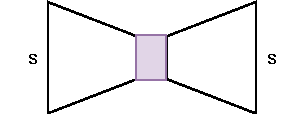
\includegraphics[width=\linewidth]{img/very_simple_autoencoder.pdf}
		\caption{Simple autoencoder}
		\label{subfig:repr_learner_simple_autoencoder}
	\end{subfigure}%
	~ 
	\begin{subfigure}{0.45\columnwidth}
		\centering
		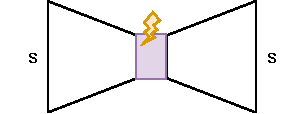
\includegraphics[width=\linewidth]{img/variational_autoencoder.pdf}
		\caption{Variational autoencoder}
		\label{subfig:repr_learner_vae}
	\end{subfigure}
	\begin{subfigure}{0.5\columnwidth}
		\centering
		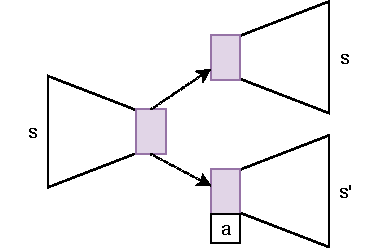
\includegraphics[width=\linewidth]{img/janus.pdf}
		\caption{Janus}
		\label{subfig:repr_learner_janus}
	\end{subfigure}%
	~ 
	\begin{subfigure}{0.5\columnwidth}
		\centering
		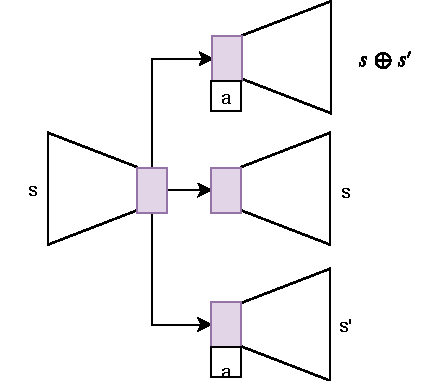
\includegraphics[width=\linewidth]{img/cerberus.pdf}
		\caption{Cerberus}
		\label{subfig:repr_learner_cerberus}
	\end{subfigure}
	\caption{Network architectures of of representation learner, where $s$ and $s'$ indicate current and next state respectively, and $a$ indicates the action leading from $s$ to $s$. 
	The layers marked in purple are the latent representations to be used as the basis of later transfer learning. 
	The arrows indicate a straight copy from source to target.
	}
	\label{fig:repr_learner}
\end{figure}

\subsubsection{Simple and Variational Autoencoder}
The simplest representation learner is an autoencoder, which compresses and reconstructs the current state representation. 
Figure \ref{subfig:repr_learner_simple_autoencoder} illustrates the simple autoencoder, and \ref{subfig:repr_learner_vae} the variational autoencoder (VAE). 
%The VAE . 
One theoretical drawback of such structure for representation learning is that
since the latent space only aims at compression, it is not necessarily a useful basis for transfer learning.
The upcoming architectures account for this.

\subsubsection{Janus}
To create more guidance in the construction of the latent space, we add another sub-network to capture the dynamics of the environment. 
As shown in Figure \ref{subfig:repr_learner_janus},
in addition to reconstructing the current state, we also append the action in latent space and seek to use this combination to predict the next state.
The hypothesized effect of this approach is that the latent representation is incentivized to preserve transition dynamics in the environment, and therefore is a more meaningful abstraction of the task.

\subsubsection{Cerberus}
Compared to Janus, the Cerberus architecture contains one more output sub-network, which aims to predict the difference between the current and next state. 
By only predicting the differences instead of the next state in its entirety, focus is placed on the change caused by the action taken.
We expect this to be especially useful when the changes between consecutive states are small relative to the entire state representation.
The network architecture is shown in Figure \ref{subfig:repr_learner_cerberus}.  

\subsection{Policy Learners}
Based on the latent space constructed by the representation learner, the policy learner trains an RL agents to complete the given task.
%More specifically, take the output

%\subsubsection{Table-based(?)}

\subsubsection{Deep Q-Network}
One of the drawbacks of table-based Q-learning occurs in environments with large state spaces.
Maintaining and updating the values of all possible states is memory intensive requires a great amount of training data.
An alternative that avoids this problem is function approximation. 
We use Deep Q-Network (DQN) \citep{DQN}, which is a Q-learning algorithm that uses deep neural networks to approximate the Q values of states.

Experience replay is used to improve the learning process in DQN. 
This mechanism stores the situations that the agent previously encountered as ``memories'' and randomly samples them to train the network. 
The sampling of memories is meant to remove correlation between training instances and facilitate learning.
Furthermore, prioritized memory \citep{prioritized_memory} is used to more frequently learn from situations that caused more loss previously. %by adjusting sampling weights.

%some memory is more important, depending on loss, give more prio to the ones that have major loss. Try to choose the ones causing more loss. 


\subsubsection{Double Deep Q-Network}
The double Deep Q-Network \citep{DDQN} is an improvement to DQN that stabilizes the target Q-values to be predicted. 
More specifically, the target is kept fixed for a certain number of steps, contrary to in DQN where it changes every step.
\iffalse
\begin{itemize}
	\item DDQN  also has prioritized memory 
	%Dueling DQN \citep{DuelingDQN}: state value, mix between q=learning and state action.
	\item DQN update policy every time. 
	\item continuously changing policy, estimate q-value changes every time.
	target network updated every 100 steps. prediction of q-values is fixed. otherwise there is ``more bias''?
\end{itemize}
\fi
The Double DQN also uses prioritized memory.

\subsection{Integrating Representation and Policy Learners}
The interaction between the representation leaner and policy learner can occur in two ways depending on the execution sequence of the two learning processes.

\begin{figure}[ht!]
	\centering
	\begin{subfigure}{\columnwidth}
		\centering
		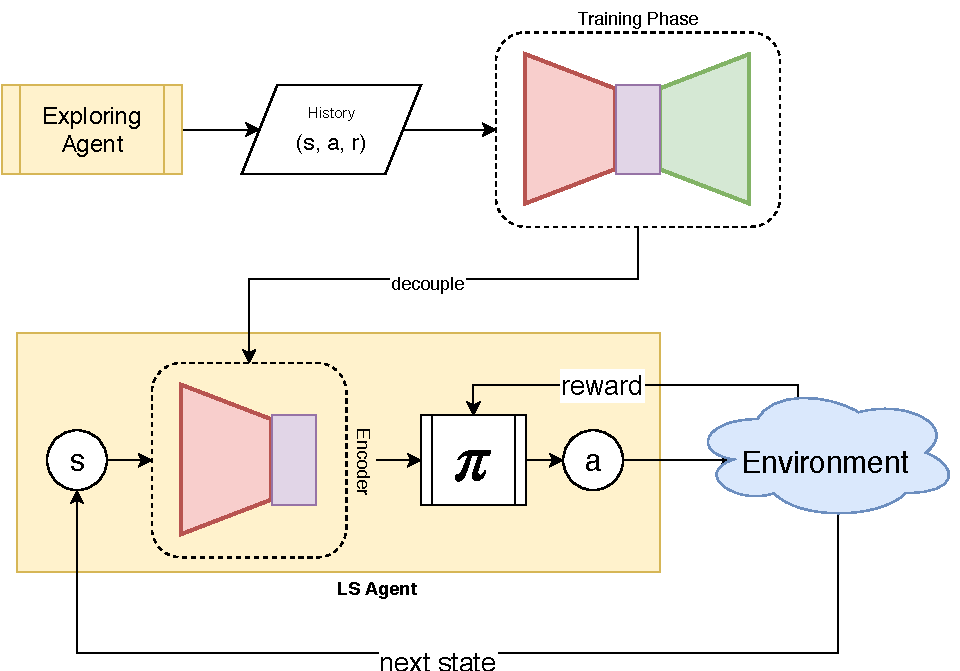
\includegraphics[width=\linewidth]{img/history.pdf}
		\caption{Illustration of the history approach, where the representation learner is first trained and the policy learner uses the encoding produced by trained representation learner to operate in the environment.}
		\label{subfig:approach_history}
	\end{subfigure}%
	
	\begin{subfigure}{\columnwidth}
		\centering
		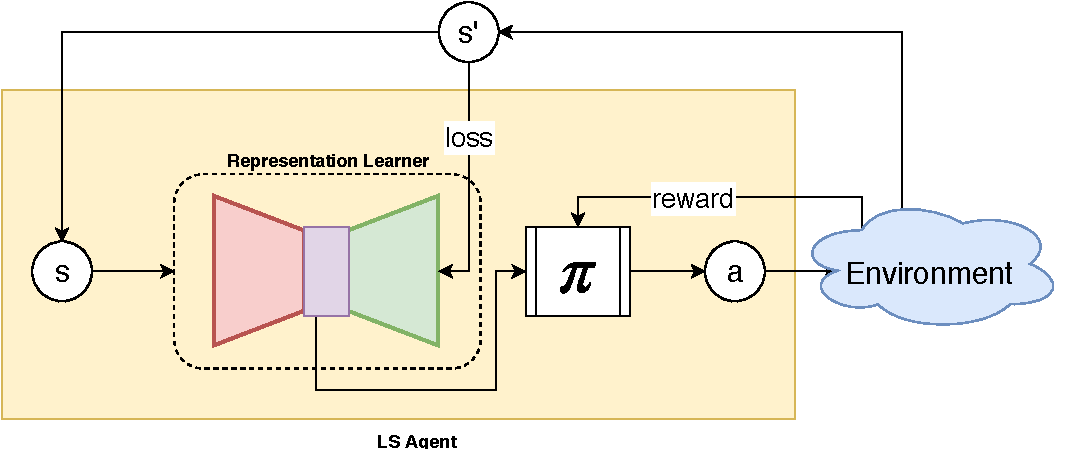
\includegraphics[width=\linewidth]{img/parallel.pdf}
		\caption{Illustration of the parallel approach, where the representation and policy learners are trained simultaneously as the RL agent operates in the environment.}
		\label{subfig:approach_parallel}
	\end{subfigure}
	\caption{Illustrations of how the representation and policy learners are integrated.
	}
	\label{fig:approaches}
\end{figure}

\subsubsection{History Approach}
As the name indicates, the history approach first creates a collection of states, actions and rewards by randomly exploring in the environment.
The representation learner is then trained based on the collected history.
Once learning completes, the policy learner is trained based on the encoding of the representation learner.
In this approach, the representation and policy learning are sequential and decoupled. 

\subsubsection{Parallel Approach}
In the parallel approach, the representation and policy learners are trained simultaneously.
As the RL agent explores the environment, it chooses an action based on the the encoded representation of the current state.
After executing the chosen action, the RL observes the new state and reward, which provide feedback to the representation and policy learners for their loss calculation respectively.
The loss of the policy learner is further back-propagated to the representation learner.

\subsection{Multi-task Learning}
\begin{itemize}
	\item structure easy to incorporate MTL
	\item every time randomly choose an env
	\item save previously seen training instances in experience stacks
\end{itemize}